\documentclass[11pt]{article}
\usepackage[table]{xcolor}
\usepackage[margin=1in]{geometry}
\usepackage{amsmath}
\usepackage{graphicx}

\usepackage{setspace}

\usepackage{amssymb}
\usepackage{epstopdf}
\usepackage{inputenc}

\usepackage{dashrule}
\usepackage{float}
\usepackage{hyperref}
\usepackage{url}
\usepackage{mwe}
\usepackage{caption}
\usepackage{multirow}
\usepackage{booktabs}
\usepackage{minted}

\usepackage[backend=biber,style=authoryear-icomp]{biblatex}
\usepackage[toc]{appendix}
\usepackage[acronym]{glossaries}

\addbibresource{references.bib}

\hypersetup{ linktoc=all}
\graphicspath{ {./images/} }


\begin{document}
\title{%
	\bf Biologically Inspired Computing\\ 
    \large - \\
    Training an Artificial Neural Network\\
     using Particle Swarm Optimisation\\
     -\\
     \url{https://www2.macs.hw.ac.uk/~sf52/Bio-Comp-docs/html/index.html}}

\author{
	Sam Fay-Hunt | \texttt{sf52@hw.ac.uk}\\
	Kamil Szymczak | \texttt{ks83@hw.ac.uk}
}

\maketitle
\thispagestyle{empty}
\pagebreak

\tableofcontents
\thispagestyle{empty}
\pagebreak


\setcounter{page}{1}

\section{Introduction}
This report details our reationale when developing our Artificial Neural Network (ANN) and Particle Swarm Optimisation (PSO) implementations, A description of the methodology we employed, and the results from the experiments we performed to gain insight into the factors that can effect the quality of PSO.

Our solution is written in Python, heavily utilising numpy, pandas and the python standard libraries, additionally we made use of matplotlib for plotting graphs and SKlearn to split the data into training and testing sets.
We used an OOP approach to keep the project organised so we could maintain the fairly large codebase, this also neatly decoupled the ANN and the PSO modules.
We used jupyter notebooks to demonstrate how to use our codebase, and to present our findings.
We used sphinx to generate documentation of the sourcecode, links to our \href{https://www2.macs.hw.ac.uk/~sf52/Bio-Comp-docs/html/index.html}{documentation} are included throughout this report to help provide context.

\begin{figure}[H]
    \begin{center}
        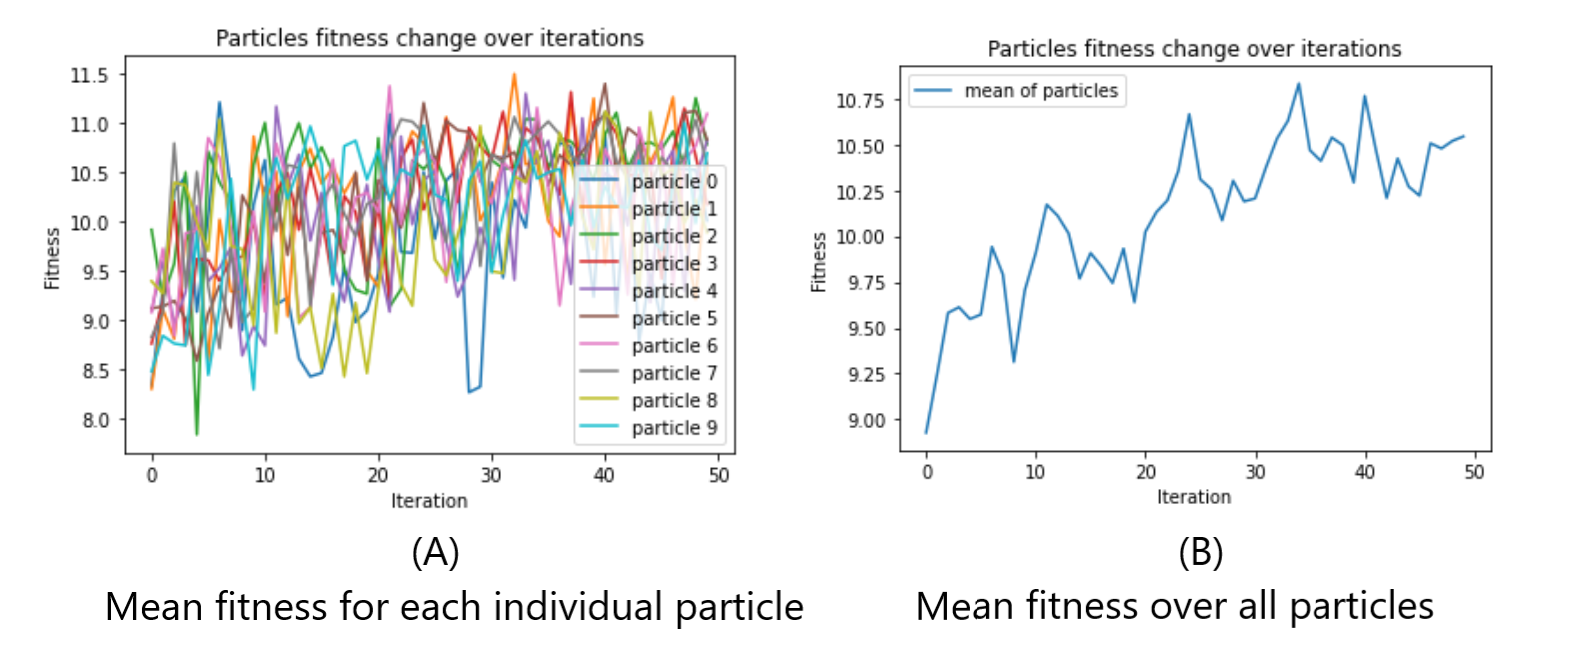
\includegraphics[width=1\textwidth]{comples_pso_combined.png} 
    \end{center}
    
    \caption{Learning PSO hyperparameters with PSO for the complex dataset.}
    \label{fig:complexpsolearning}   
\end{figure}

\section{Development Rationale}
Our rationale was to create 2 submodules: \href{https://www2.macs.hw.ac.uk/~sf52/Bio-Comp-docs/html/Coursework.ANNModel.html}{ANNModel} and \href{https://www2.macs.hw.ac.uk/~sf52/Bio-Comp-docs/html/Coursework.PSO.html}{PSO} that could be used to build a fully connected neural network or perform PSO independently.
We wanted the submodules to be completely decoupled to allow PSO to work on arbitrary Optimisation problems.\\

\noindent~ANNModel is only able to create a fully connected neural network, we made this descision to simplify the process of vectorizing the parameters of the network for optimisation with PSO, this also made converting the vector back into a model easier.

The ANNModel’s design was inspired by TensorFlow \& Keras~\autocite{kerasKerasDocumentationModel,tensorflowModuleTfKeras}, specifically when defining the shape of the neural network. For example you can instantiate the empty network, define the input and result vectors, the layers and then, finally, compile the model.
Once compiled you can perform a \href{https://www2.macs.hw.ac.uk/~sf52/Bio-Comp-docs/html/Coursework.ANNModel.html?highlight=one_pass#Coursework.ANNModel.model.ANN.one_pass}{single pass} on the model with either random weights or activations, biases and weights defined by a vector.\\

\noindent~The PSO class utilises a Particle class to abstract away some complexity.
To use the PSO class define the hyperparameters in the constructor (as described in the \href{https://www2.macs.hw.ac.uk/~sf52/Bio-Comp-docs/html/Coursework.PSO.html?highlight=pso#Coursework.PSO.pswarm.PSO}{documentation}), and then specify the fitness function and search dimensions for PSO. \\

\noindent~We created an interface for PSO Called \href{https://www2.macs.hw.ac.uk/~sf52/Bio-Comp-docs/html/Coursework.PSO.html?highlight=optimisable#Coursework.PSO.interface.Optimisable}{Optimisable}, any class that properly implements this interface can be used with our PSO implementation. 
The beauty of this technique is that it allowed us to implement this interface on our PSO class and construct a (PSO) optimiser for our PSO hyperparameters for a specific model shape, for clarity we refer to this outer PSO optimiser as ``meta-PSO'' and the inner PSO optimiser as ``inner-PSO''.

This interface also allowed us to create some wrapper classes(PSOHistory, PSOFittest) that can store detailed data about all the hyperparameter settings of the model being optimised.
Figure~\ref{fig:dimensionVec} shows the definitions of  the hyperparameters and boundaries that our meta PSO algorithm searches over. 

\begin{figure}[h]
    \caption{A list describing the dimensions and boundaries that PSO will search over. See the documentation for more information~\autocite{fay-huntBiologicallyInspiredComputation}.}
    \label{fig:dimensionVec}
    \begin{minted}{python}
        def dimension_vec(self):
            swarm_size = (10, 100)
            informants = (4, 8)
            alpha = (0.01, 2.0)
            beta = (0.01, 2.0)
            gamma = (0.01, 2.0)
            delta = (0.01, 2.0)
            epsilon = (0.01, 2.0)
            return [swarm_size, informants, alpha, beta, gamma, delta, epsilon]
    \end{minted}
\end{figure}


\newpage
\section{Testing Methodology}

As explained in the previous section, we used a method to find good PSO hyperparameters by applying PSO to another PSO that itself tries to optimize our ANN for a defined dataset.
This allowed us to investigate a wide search space of potential optimal hyperparameters for the PSO that was used to optimize the given ANN.\\

\noindent\textbf{Testing steps:}
\begin{enumerate}
    \item Run the Meta\_pso notebook with each dataset and record the resulting vectors.
    \item Copy the vectors from Meta\_pso to the evaluation notebook.
    \item For each pair of datasets from Meta\_pso set the corresponding training/testing data, the decimal places to compare, the PSO, and ANN parameters.
    \item Run the tests and record the results.
\end{enumerate}



\newpage
\section{Results}

\begin{table}[H]
    \begin{tabular}{@{}|cl|l|lll|@{}}
    \toprule
    \multicolumn{1}{|l}{}                        & Experiment                                                                                   & Data  & Fitness & Loss  & Score* \\ \midrule
    \multicolumn{1}{|c|}{\multirow{4}{*}{Cubic}} & \multirow{2}{*}{Best ANN params}                                                             & Train & 4437    & 0     & 97\%   \\ \cmidrule(l){3-6} 
    \multicolumn{1}{|c|}{}                       &                                                                                              & Test  & 6847    & 0     & 100\%  \\ \cmidrule(l){2-6} 
    \multicolumn{1}{|c|}{}                       & \multirow{2}{*}{\begin{tabular}[c]{@{}l@{}}10 run mean from \\ best PSO params\end{tabular}} & Train & 47      & 0.028 & 12\%   \\ \cmidrule(l){3-6} 
    \multicolumn{1}{|c|}{}                       &                                                                                              & Test  & 61      & 0.022 & 9\%    \\ \bottomrule
    \multicolumn{1}{|c|}{\multirow{4}{*}{Linear}} & \multirow{2}{*}{Best ANN params}                                                             & Train & 3.005e+17 & 0     & 100\%  \\ \cmidrule(l){3-6} 
    \multicolumn{1}{|c|}{}                        &                                                                                              & Test  & 3.380e+17 & 0     & 100\%  \\ \cmidrule(l){2-6} 
    \multicolumn{1}{|c|}{}                        & \multirow{2}{*}{\begin{tabular}[c]{@{}l@{}}10 run mean from \\ best PSO params\end{tabular}} & Train & 223       & 0.033 & 31\%   \\ \cmidrule(l){3-6} 
    \multicolumn{1}{|c|}{}                        &                                                                                              & Test  & 219       & 0.029 & 34\%   \\ \bottomrule
    \multicolumn{1}{|c|}{\multirow{4}{*}{Tanh}} & \multirow{2}{*}{Best ANN params}                                                             & Train & 236154  & 0     & 100\%  \\ \cmidrule(l){3-6} 
    \multicolumn{1}{|c|}{}                      &                                                                                              & Test  & 74997   & 0     & 100\%  \\ \cmidrule(l){2-6} 
    \multicolumn{1}{|c|}{}                      & \multirow{2}{*}{\begin{tabular}[c]{@{}l@{}}10 run mean from \\ best PSO params\end{tabular}} & Train & 49      & 0.078 & 26\%   \\ \cmidrule(l){3-6} 
    \multicolumn{1}{|c|}{}                      &                                                                                              & Test  & 55      & 0.101 & 22\%   \\ \bottomrule
    \multicolumn{1}{|c|}{\multirow{4}{*}{Sine}} & \multirow{2}{*}{Best ANN params}                                                             & Train & 487.8   & 0.002 & 31\%   \\ \cmidrule(l){3-6} 
    \multicolumn{1}{|c|}{}                      &                                                                                              & Test  & 459.3   & 0.002 & 39\%   \\ \cmidrule(l){2-6} 
    \multicolumn{1}{|c|}{}                      & \multirow{2}{*}{\begin{tabular}[c]{@{}l@{}}10 run mean from \\ best PSO params\end{tabular}} & Train & 12.28   & 0.083 & 11\%   \\ \cmidrule(l){3-6} 
    \multicolumn{1}{|c|}{}                      &                                                                                              & Test  & 12.02   & 0.086 & 8\%    \\ \bottomrule
    \multicolumn{1}{|c|}{\multirow{4}{*}{Complex}} & \multirow{2}{*}{Best ANN params}                                                             & Train & 20.17   & 0.05  & 9\%    \\ \cmidrule(l){3-6} 
    \multicolumn{1}{|c|}{}                         &                                                                                              & Test  & 16.05   & 0.062 & 18\%   \\ \cmidrule(l){2-6} 
    \multicolumn{1}{|c|}{}                         & \multirow{2}{*}{\begin{tabular}[c]{@{}l@{}}10 run mean from \\ best PSO params\end{tabular}} & Train & 7.83    & 0.129 & 12\%   \\ \cmidrule(l){3-6} 
    \multicolumn{1}{|c|}{}                         &                                                                                              & Test  & 20.96   & 0.049 & 17\%   \\ \bottomrule
    \multicolumn{1}{|c|}{\multirow{4}{*}{XOR}} & \multirow{2}{*}{Best ANN params}                                                             & Train & 9096925098444960 & 0     & 100\%  \\ \cmidrule(l){3-6} 
    \multicolumn{1}{|c|}{}                     &                                                                                              & Test  & 16.05            & 0     & 100\%  \\ \cmidrule(l){2-6} 
    \multicolumn{1}{|c|}{}                     & \multirow{2}{*}{\begin{tabular}[c]{@{}l@{}}10 run mean from \\ best PSO params\end{tabular}} & Train & 299545           & 0.135 & 85\%   \\ \cmidrule(l){3-6} 
    \multicolumn{1}{|c|}{}                     &                                                                                              & Test  & 263010           & 0.109 & 91\%   \\ \bottomrule
    \end{tabular}
    \caption{Table of results, showing the scores from the best ANN parameters from meta-PSO, and the mean best scores from an optimiser using the hyperparameters discovered in meta-PSO }
    \label{tab:ExperimentResults}
\end{table}

\section{Conclusion}

\subsection{Discussion}

Flaws in testing:
\begin{itemize}
    \item We use a fixed model structure for our neural network during testing, cannot generalise to other models.
    \item The fitness function we used was simply 1/loss, this was easy to implement but may have impacted the ability of PSO to escape local maximum. In future a linear fitness value may have been preferred.
    \item During meta-PSO we only took the mean of 10 inner-PSO runs to evaluate the fitness of each inner-PSO hyperparameter configuration. More would have been better, but impractical in terms of time.
\end{itemize}

\begin{itemize}
    \item The best ANN hyperparameters we observed appeared to be a result of running at least 12.5 million different ANN hyperparameter configurations each time we ran meta-PSO in an attempt to optimise the inner-PSO hyperparameters for a given dataset.
    \item This might suggest the highest performing ANN hyperparameters discovered during our search for good PSO hyperparameters  were more due to reinitialising PSO so many times than actually finding some really good PSO hyperparameters.
    \item We frequently observed PSO getting stuck in local maximum, this is reflected by the disparity in table~\ref{tab:ExperimentResults} between the 10 run mean results and the results recorded from the best found during meta-PSO 
    \item meta-PSO found a mean swarm size of 74 particles, this somewhat supports the observation that this is more of a brute force approach and (this implemenation) is very wasteful in terms of computation. 
    \item Poor computational performance of our implementation (Memory access bottlenecks?)
\end{itemize}

\subsection{Further work}
From the experimental results we have observed we feel future experiments should look closer at other fitness evaluation techniques. 
An investigation into different hyperparameter search dimensions for both the ANN model and PSO would be interesting, some hyperparameters were found very quickly and it may be worth investigating if we could freeze those once they are found during optimiser runtime and reduce the search dimensions (careful consideration should be made with getting stuck in local maxima here). 

A proper benchmark suite should be implemented to identify the serious bottlenecks in computation and memory access so we can begin to address them, and run more comprehensive experiments within a reasonable timeframe.
Likewise a unit testing suite would be helpful in idientifying any remaining bugs in this codebase, and may also provide some insight into the performance bottlenecks.

Implementing PSO visualization tools to view how the hyperparameters are affecting the fitness in real-time would provide more insight into what is going on with particles during optimization. This information might allow us to identify hyperparameters that tend to result in the particle being caught in local maxima.

\subsection{Finally}
Findings in~\autocite{garcia-nietoWhySixInformants2012,garcia-nietoEmpiricalComputationQuasioptimal2011} indicate that 6 to 8 informants is generally a good number of informants that each particle should have. 
Our own findings support this.

\pagebreak
\appendix

\section{References}
\printbibliography

\end{document}
